% TMLR submission template — built by Pandoc from Markdown source.
\documentclass[10pt]{article}
\usepackage{tmlr}
% For camera-ready: \usepackage[accepted]{tmlr}
% For preprint: \usepackage[preprint]{tmlr}

\usepackage[T1]{fontenc}
\usepackage[utf8]{inputenc}
\usepackage{textcomp}

% Unicode character mappings for pdflatex
\DeclareUnicodeCharacter{00B0}{\textdegree}
\DeclareUnicodeCharacter{00B2}{\textsuperscript{2}}
\DeclareUnicodeCharacter{00D7}{\ensuremath{\times}}
\DeclareUnicodeCharacter{0394}{\ensuremath{\Delta}}
\DeclareUnicodeCharacter{2013}{--}
\DeclareUnicodeCharacter{2019}{'}
\DeclareUnicodeCharacter{201C}{``}
\DeclareUnicodeCharacter{201D}{''}
\DeclareUnicodeCharacter{2192}{\ensuremath{\rightarrow}}
\DeclareUnicodeCharacter{21D2}{\ensuremath{\Rightarrow}}
\DeclareUnicodeCharacter{2248}{\ensuremath{\approx}}

\usepackage{amsmath,amssymb}
\usepackage{graphicx}
\setkeys{Gin}{width=\linewidth,height=0.9\textheight,keepaspectratio}
\usepackage{booktabs}
\usepackage{longtable}
\usepackage{array}
\usepackage{float}
\usepackage{caption}
\usepackage{xcolor}
\usepackage{hyperref}
\usepackage{url}
\usepackage{calc}

\hypersetup{
  colorlinks=true,
  linkcolor=blue,
  citecolor=blue,
  urlcolor=blue
}

% Pandoc emits \tightlist for compact lists.
\providecommand{\tightlist}{%
  \setlength{\itemsep}{0pt}\setlength{\parskip}{0pt}}

% Bibliography handled by natbib + bibtex (tmlr.bst).

\usepackage{color}
\usepackage{fancyvrb}
\newcommand{\VerbBar}{|}
\newcommand{\VERB}{\Verb[commandchars=\\\{\}]}
\DefineVerbatimEnvironment{Highlighting}{Verbatim}{commandchars=\\\{\}}
% Add ',fontsize=\small' for more characters per line
\newenvironment{Shaded}{}{}
\newcommand{\AlertTok}[1]{\textcolor[rgb]{1.00,0.00,0.00}{\textbf{#1}}}
\newcommand{\AnnotationTok}[1]{\textcolor[rgb]{0.38,0.63,0.69}{\textbf{\textit{#1}}}}
\newcommand{\AttributeTok}[1]{\textcolor[rgb]{0.49,0.56,0.16}{#1}}
\newcommand{\BaseNTok}[1]{\textcolor[rgb]{0.25,0.63,0.44}{#1}}
\newcommand{\BuiltInTok}[1]{\textcolor[rgb]{0.00,0.50,0.00}{#1}}
\newcommand{\CharTok}[1]{\textcolor[rgb]{0.25,0.44,0.63}{#1}}
\newcommand{\CommentTok}[1]{\textcolor[rgb]{0.38,0.63,0.69}{\textit{#1}}}
\newcommand{\CommentVarTok}[1]{\textcolor[rgb]{0.38,0.63,0.69}{\textbf{\textit{#1}}}}
\newcommand{\ConstantTok}[1]{\textcolor[rgb]{0.53,0.00,0.00}{#1}}
\newcommand{\ControlFlowTok}[1]{\textcolor[rgb]{0.00,0.44,0.13}{\textbf{#1}}}
\newcommand{\DataTypeTok}[1]{\textcolor[rgb]{0.56,0.13,0.00}{#1}}
\newcommand{\DecValTok}[1]{\textcolor[rgb]{0.25,0.63,0.44}{#1}}
\newcommand{\DocumentationTok}[1]{\textcolor[rgb]{0.73,0.13,0.13}{\textit{#1}}}
\newcommand{\ErrorTok}[1]{\textcolor[rgb]{1.00,0.00,0.00}{\textbf{#1}}}
\newcommand{\ExtensionTok}[1]{#1}
\newcommand{\FloatTok}[1]{\textcolor[rgb]{0.25,0.63,0.44}{#1}}
\newcommand{\FunctionTok}[1]{\textcolor[rgb]{0.02,0.16,0.49}{#1}}
\newcommand{\ImportTok}[1]{\textcolor[rgb]{0.00,0.50,0.00}{\textbf{#1}}}
\newcommand{\InformationTok}[1]{\textcolor[rgb]{0.38,0.63,0.69}{\textbf{\textit{#1}}}}
\newcommand{\KeywordTok}[1]{\textcolor[rgb]{0.00,0.44,0.13}{\textbf{#1}}}
\newcommand{\NormalTok}[1]{#1}
\newcommand{\OperatorTok}[1]{\textcolor[rgb]{0.40,0.40,0.40}{#1}}
\newcommand{\OtherTok}[1]{\textcolor[rgb]{0.00,0.44,0.13}{#1}}
\newcommand{\PreprocessorTok}[1]{\textcolor[rgb]{0.74,0.48,0.00}{#1}}
\newcommand{\RegionMarkerTok}[1]{#1}
\newcommand{\SpecialCharTok}[1]{\textcolor[rgb]{0.25,0.44,0.63}{#1}}
\newcommand{\SpecialStringTok}[1]{\textcolor[rgb]{0.73,0.40,0.53}{#1}}
\newcommand{\StringTok}[1]{\textcolor[rgb]{0.25,0.44,0.63}{#1}}
\newcommand{\VariableTok}[1]{\textcolor[rgb]{0.10,0.09,0.49}{#1}}
\newcommand{\VerbatimStringTok}[1]{\textcolor[rgb]{0.25,0.44,0.63}{#1}}
\newcommand{\WarningTok}[1]{\textcolor[rgb]{0.38,0.63,0.69}{\textbf{\textit{#1}}}}


% TMLR title
\title{Modality-Driven Search with Holistic Trace Judging for ARC-AGI-2}

% Authors hidden for anonymous submission.
% Uncomment and fill in for camera-ready.
% \author{\name Anonymous \email anonymous@example.com \\
%       \addr Anonymous Institution}

\def\month{MM}
\def\year{YYYY}
\def\openreview{\url{https://openreview.net/forum?id=XXXX}}

\begin{document}

\maketitle

\begin{abstract}
Large language models (LLMs) can generate convincing reasoning traces
for abstract reasoning tasks while still being confidently wrong. The
core challenge is therefore not only generating solutions, but reliably
distinguishing correct from incorrect solutions in the presence of
persuasive overclaiming, including within detailed traces. We introduce
a solver for ARC-AGI-2 built around two principles: (i) modality-driven
candidate generation across independent reasoning channels (text,
images, and code with tool-use) to produce diverse candidate solutions,
and (ii) context-preserving holistic judging that evaluates all
candidate traces jointly in one prompt to identify the most likely
correct outputs, including the common case on hard tasks where the
correct solution is not the majority hypothesis. On the ARC Prize
semi-private evaluation set (used for the official leaderboard), this
solver achieves 72.9\% solved at \$38.99/task --- the highest score on
the ARC-AGI-2 Verified leaderboard at the time of submission, exceeding
the next-best entry by +18.7 percentage points. On the public evaluation
set, it achieves 76.11\% solved at \$19.69/task (self-measured). We
release the full source code and document negative results showing which
common prompting and decomposition strategies reduced diversity and hurt
performance.
\end{abstract}

\hypertarget{introduction}{%
\section{Introduction}\label{introduction}}

A central challenge in applying LLMs to abstract reasoning is not just
producing candidate solutions, but \textbf{knowing what is right and
what is wrong} in a setting where models can be confidently incorrect
--- even when they provide detailed, plausible reasoning traces.
ARC-AGI-2 \citep{arcprize2024report} was designed to be \emph{easy for
humans and hard for AI}, and --- critically --- to measure both
\textbf{capability} and \textbf{efficiency} (cost).

This paper describes an approach that treats \textbf{modalities as
search operators} and uses \textbf{judging as the final selection
mechanism}: generate diverse candidate solutions across independent
reasoning channels (text, image, and code with tool-use), then select
among them using a context-preserving holistic judge that reads all
candidate traces jointly. Unlike standard self-consistency (majority
vote) or per-candidate scoring, this judge identifies correct
\emph{minority} hypotheses by comparing full reasoning traces in a
single context window --- yielding +7 solved instances over majority
vote at only 13\% of total system cost.

On the ARC Prize semi-private evaluation set, this solver achieves
\textbf{72.9\%} at \$38.99/task --- the highest score on the ARC-AGI-2
Verified leaderboard at the time of submission, exceeding the next-best
entry by +18.7 percentage points. On the public evaluation set, it
achieves \textbf{76.11\%} at \$19.69/task (self-measured). The full
source code and public-evaluation run data are released.\footnote{Anonymized
  for review.} This paper also documents negative results showing which
common prompting and decomposition strategies reduced diversity and hurt
performance.

\hypertarget{background-and-related-work}{%
\section{Background and Related
Work}\label{background-and-related-work}}

\hypertarget{arc-agi-as-a-benchmark-for-abstraction}{%
\subsection{ARC-AGI as a benchmark for
abstraction}\label{arc-agi-as-a-benchmark-for-abstraction}}

The Abstraction and Reasoning Corpus (ARC) was introduced by
\citet{chollet2019measure} as part of a broader argument for measuring
intelligence as \textbf{skill-acquisition efficiency}. ARC tasks are
framed as \textbf{few-shot input--output induction}: given a handful of
training demonstrations (pairs of grids), the solver must infer an
underlying transformation rule and apply it to a held-out test input.
The hallmark difficulty is \textbf{underspecification}: multiple
hypotheses can explain the training pairs, but only a subset will
transfer to the test instance. An illustrative task example is provided
in the appendix.

ARC-AGI-2 \citep{arcprize2024report} is a second-generation benchmark
with calibrated public, semi-private, and private evaluation splits (120
tasks each), designed to reduce susceptibility to brute-force program
search and provide a wider useful range of scores. Evaluation uses
\textbf{pass@2} scoring (two guesses permitted per test instance), and
ARC Prize emphasizes not just raw accuracy but also \textbf{efficiency}
(cost per task).

\hypertarget{related-work}{%
\subsection{Related work}\label{related-work}}

\textbf{Classical ARC solvers} treat tasks as latent programs composed
from a hand-designed DSL, relying on enumerative search over
transformation chains \citep{ferre2021arc}. These systems established
that search can compensate for weak learned priors, and motivated
ARC-AGI-2's design to be ``less brute-forcible.''

\textbf{Learned and hybrid approaches} include transduction-based
methods (directly predicting test outputs) and induction-based methods
(inferring latent programs). \citet{li2024induction} show that combining
induction and transduction can approach human-level performance on the
original ARC under their experimental setup. Other notable approaches
include latent program search \citep{bonnet2024latent}, neurally-guided
program induction \citep{ouellette2024neurally}, small transformer
models \citep{fletcherhill2024miniarc}, and 2D nGPT architectures
\citep{puget2024nGPT}. Benchmark extensions such as ConceptARC
\citep{moskvichev2023conceptarc}, ARC-GEN \citep{moffitt2025arcgen}, and
Re-ARC \citep{hodel2024rearc} address data limitations.

\textbf{Test-time compute scaling} has become a major theme in ARC
solving. Chain-of-thought prompting \citep{wei2022chain} showed that
eliciting step-by-step reasoning improves performance on complex tasks.
\citet{snell2024scaling} show that optimally allocating test-time
compute can be more effective than scaling model parameters.
\citet{akyurek2024surprising} demonstrate that updating model parameters
at test time yields strong gains on ARC-like reasoning. Self-consistency
\citep{wang2022selfconsistency} demonstrated that sampling multiple
reasoning paths and selecting the most consistent answer outperforms
single-trace inference. Tree of Thoughts \citep{yao2023tree} and Graph
of Thoughts \citep{besta2024graph} reframe inference as explicit search
over intermediate reasoning units.

\textbf{Tool-augmented reasoning} --- ReAct \citep{yao2022react}, PAL
\citep{gao2023pal}, Toolformer \citep{schick2023toolformer} --- is
directly relevant to ARC, where code synthesis serves both as a
hypothesis generator and as a source of structured intermediate
artifacts for downstream selection. Iterative refinement methods
(Self-Refine \citep{madaan2023selfrefine}, Reflexion
\citep{shinn2023reflexion}) trade tokens for improved outputs but risk
anchoring to early hypotheses.

\textbf{LLM-as-a-judge} paradigms \citep{zheng2023judging} delegate
selection to LLM evaluators, showing strong correlation with human
preferences alongside systematic biases (position, verbosity). For ARC
in particular, selection is unusually difficult because many hypotheses
fit the demonstrations yet fail on the test instance.

\hypertarget{positioning-of-this-work}{%
\subsection{Positioning of this work}\label{positioning-of-this-work}}

This approach combines three trends: (1) \textbf{hypothesis generation
as explicit search} across \emph{multiple reasoning modalities} rather
than a single representation, (2) \textbf{tool-mediated reasoning}
producing richer intermediate artifacts for downstream selection, and
(3) \textbf{judge-based selection} adapted for ARC's specific challenge
of judging \emph{generalization under underspecification}. The
distinctive element is combining heterogeneous candidate generators with
context-preserving comparison over full traces, rather than scalar
scoring or consensus compression.

\hypertarget{method}{%
\section{Method}\label{method}}

\hypertarget{core-idea-modalities-as-search-operators}{%
\subsection{Core idea: modalities as search
operators}\label{core-idea-modalities-as-search-operators}}

The solver is built around a practical observation: to solve tasks that
frontier systems \emph{do not already solve}, the correct solution is
often a \textbf{minority hypothesis}. Therefore, the solver
intentionally creates many \emph{independent} candidate solutions across
heterogeneous reasoning modalities (text, image, and code), maximizing
the probability that at least one candidate captures a genuinely novel
hypothesis. Each modality provides a structurally different
representation of the same task, which empirically produces candidates
that cluster differently (Section 4).

\hypertarget{pipeline-overview}{%
\subsection{Pipeline overview}\label{pipeline-overview}}

Figure 1 shows the end-to-end pipeline. For each ARC task:

\begin{figure}
\centering
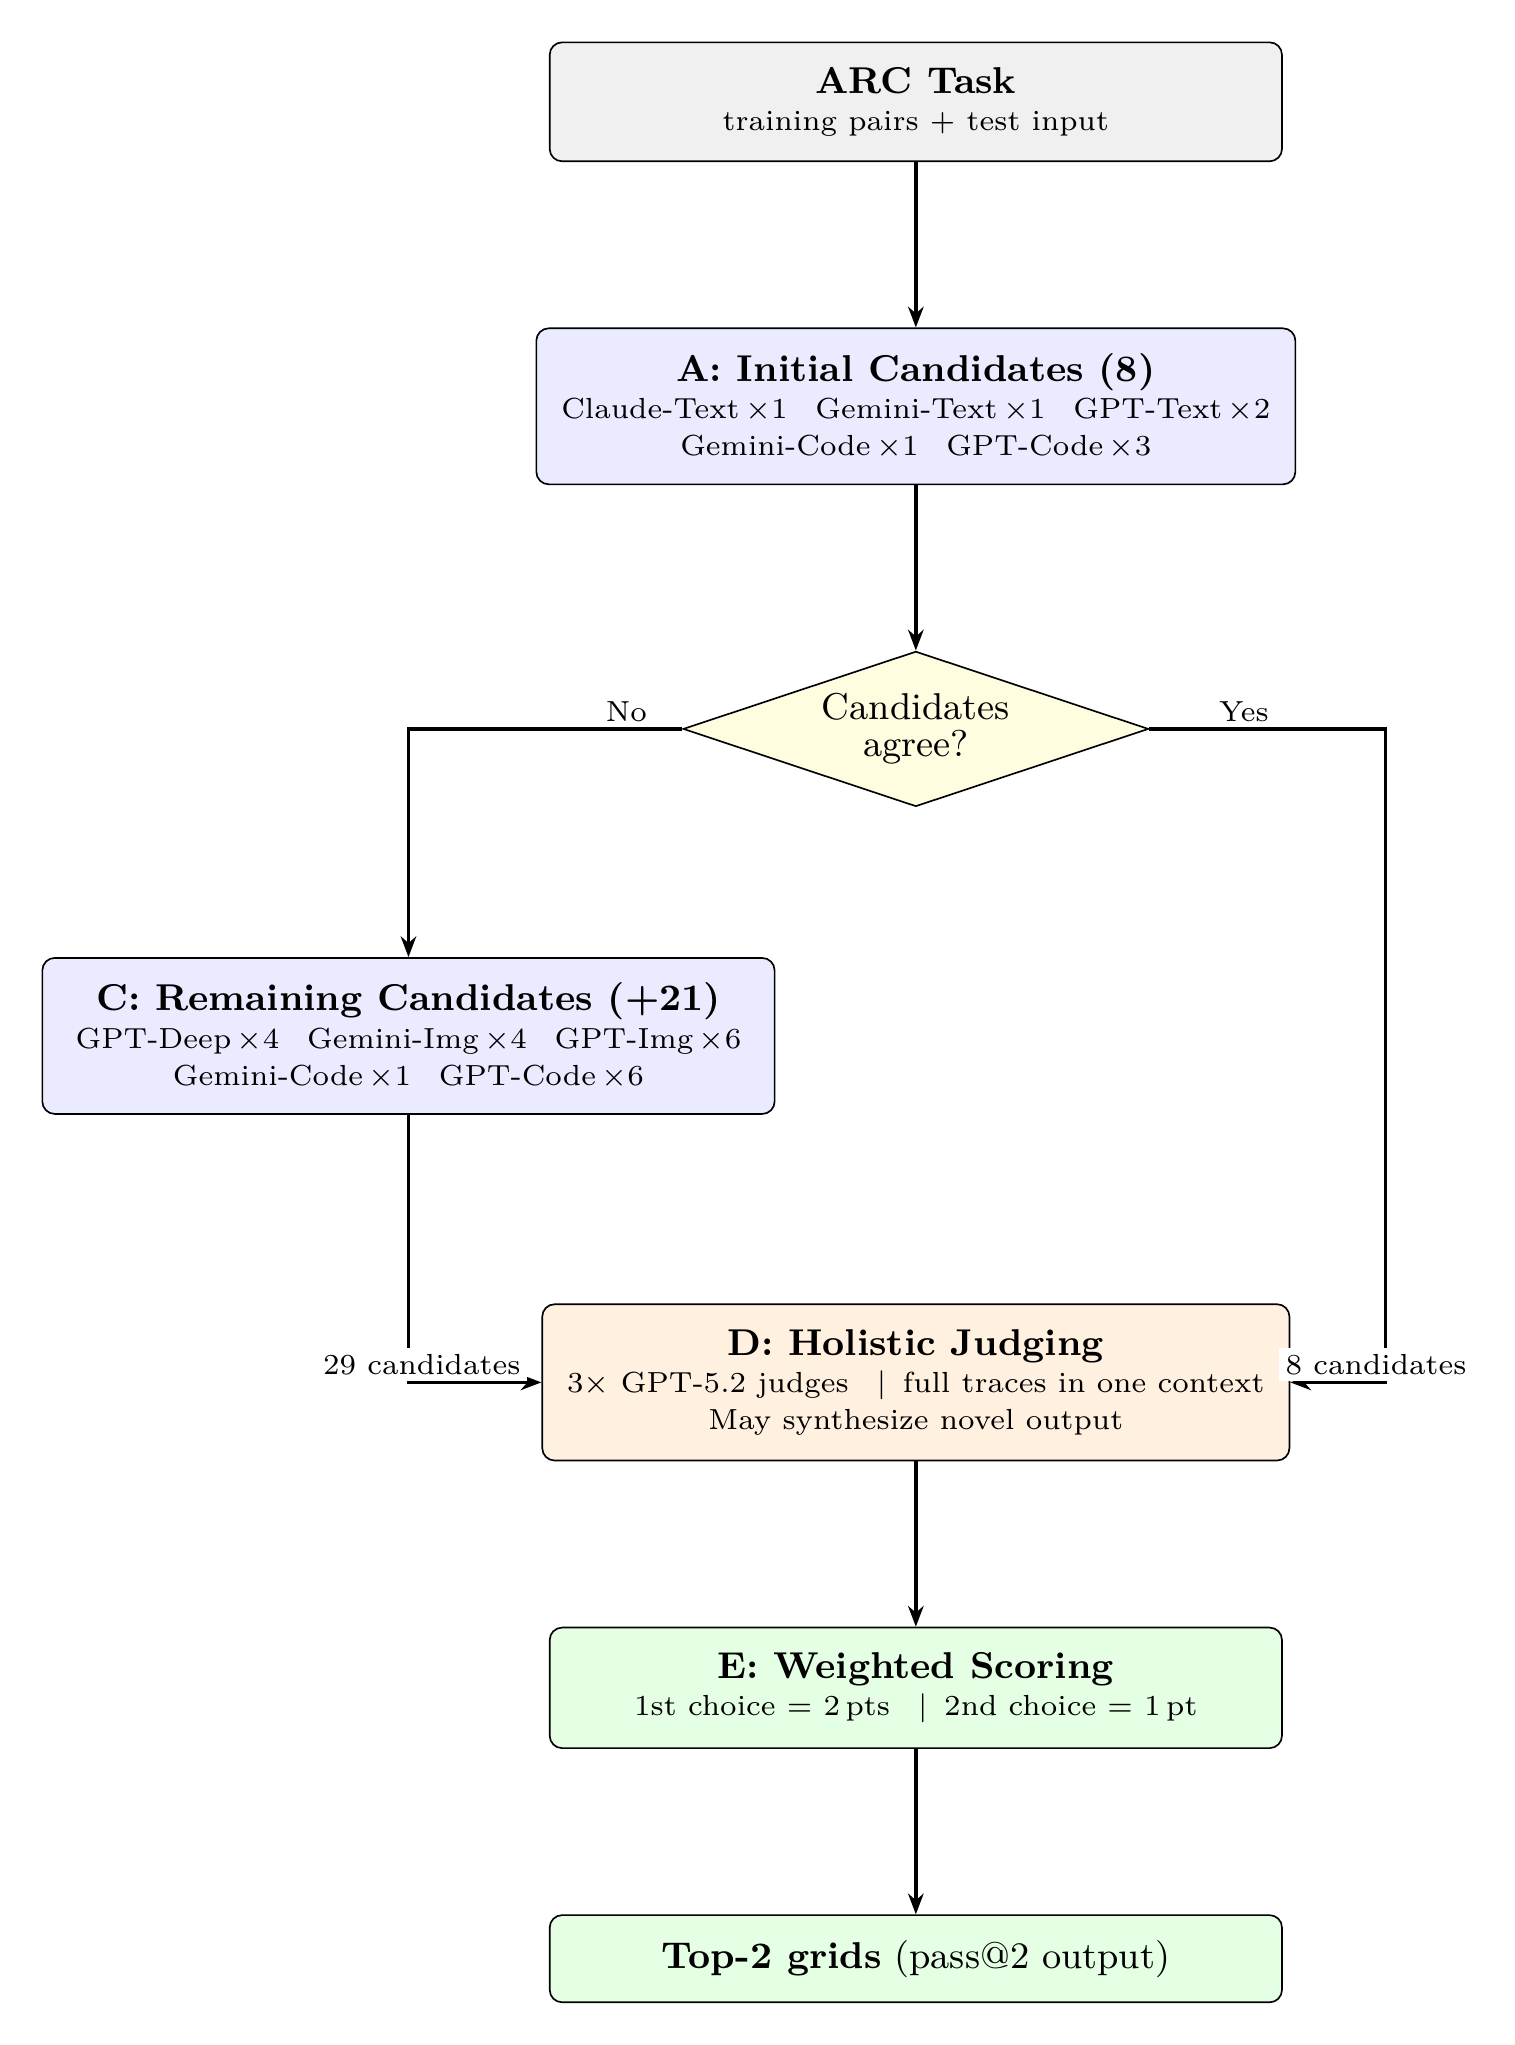
\includegraphics{figures/pipeline.png}
\caption{Solver pipeline: candidate generation with adaptive early
stopping, holistic judging, and weighted scoring.}
\end{figure}

\begin{enumerate}
\def\labelenumi{\arabic{enumi}.}
\item
  \textbf{Candidate generation (up to 29 candidates).} Run
  modality-specific solvers across text, image, and code reasoning
  channels. Each candidate produces one output grid and a reasoning
  trace; for code candidates, this includes iterative tool calls and
  execution logs. If early-stage candidates show strong agreement, the
  system terminates early and skips remaining modalities (adaptive early
  stopping).
\item
  \textbf{Holistic judging (3 parallel judges).} Concatenate all
  candidate traces into a single long-context prompt (30k--80k tokens)
  and ask a judge model to identify the top-2 most likely correct
  candidates (or propose a synthesis), explain why other clusters are
  wrong, and output the final grids.
\item
  \textbf{Weighted scoring.} Each judge's first choice receives 2 points
  and second choice receives 1 point. The two distinct output grids with
  the highest total score become the solver's pass@2 guesses.
\end{enumerate}

\hypertarget{candidate-generation}{%
\subsection{Candidate generation}\label{candidate-generation}}

Candidate generation uses three foundation models --- \textbf{Gemini 3
Preview}, \textbf{GPT-5.2}, and \textbf{Claude Opus 4.5} --- across
three modality families. The full configuration (29 generators; see
appendix for details) groups candidates as follows:

\begin{itemize}
\tightlist
\item
  \textbf{Text (8 candidates):} Standard text prompting with a minimal
  prompt (see appendix) across multiple models, plus a ``deep think''
  configuration that allocates a larger reasoning budget. The prompt
  deliberately avoids prescribed reasoning templates to maximize
  hypothesis diversity.
\item
  \textbf{Image (10 candidates):} Grids are rendered as annotated images
  alongside the instruction prompt (example rendering in the appendix).
  Renderings are intentionally \textbf{imprecise} --- slightly distorted
  rather than pixel-perfect --- because imprecision empirically
  encourages models to reason about shapes and spatial relationships at
  a higher level of abstraction rather than falling back to cell-by-cell
  numerical reasoning.
\item
  \textbf{Code (11 candidates):} Program synthesis via two regimes: (i)
  \emph{tool-integrated} code generation with iterative sandbox
  execution and debugging, and (ii) \emph{one-shot} code generation
  without execution feedback. Tool-integrated generation produces rich
  intermediate artifacts consumed by the holistic judge.\footnote{The
    ARC Prize semi-private evaluation uses OpenAI's zero-data-retention
    (ZDR) API mode, which disables tool calls. For that run,
    tool-integrated candidates were replaced with one-shot code
    generation.}
\end{itemize}

\hypertarget{holistic-judging}{%
\subsection{Holistic judging}\label{holistic-judging}}

The key insight is that \textbf{having all context together beats
abstracting traces into scores}. Three alternative judging approaches
were tested:

\begin{enumerate}
\def\labelenumi{\arabic{enumi}.}
\tightlist
\item
  \textbf{Logic judge (failed):} scoring candidates by reasoning
  consistency. Failure mode: candidates can be ``logical'' yet overfit
  to training pairs.
\item
  \textbf{Consistency judge (partial):} rewarding themes that repeat
  across candidates. Failure mode: rewards the majority cluster, but the
  correct solution on hard tasks is often a minority hypothesis.
\item
  \textbf{Holistic judge (final):} providing \emph{all traces together}
  and asking the judge to pick the top-2 candidates. This lets the judge
  detect subtle but decisive differences between near-identical
  hypotheses.
\end{enumerate}

The holistic judge can be understood as an \textbf{anti-consistency}
mechanism: it is designed to override the plurality answer when
trace-level reasoning suggests a minority candidate better generalizes
to the test instance. Self-consistency \citep{wang2022selfconsistency}
selects the most common answer --- effective when the majority is
correct. On ARC-AGI-2, the majority is often \emph{wrong} on the hardest
tasks, making consistency-based selection a liability.

All three judges use \textbf{GPT-5.2} (x-high reasoning). A mixed-model
ensemble was tested but three homogeneous GPT-5.2 judges outperformed
the mixed configuration. The judge prompt (detailed in the appendix)
provides all candidate traces and outputs, and asks for a
``meta-conclusion'' without instructing the judge to prefer majority or
minority answers. Each candidate's content block contains the full
reasoning trace --- for text/image candidates, the chain-of-thought
response; for code candidates, the complete iterative tool-use trace
including intermediate program drafts, execution outputs, and debugging
steps.

\textbf{Synthesis.} The judge may also propose a \textbf{novel solution}
not identical to any candidate output, recombining correct subcomponents
of multiple flawed candidates. This matters on tasks where no single
candidate is fully correct but multiple candidates contain partial
truths.

\textbf{Known limitations.} Candidate order is not shuffled between
judge runs, which could introduce position bias. The judge may also
exhibit verbosity and format biases \citep{zheng2023judging}. No
debiasing is applied in the current implementation.

\hypertarget{experiments-and-results}{%
\section{Experiments and Results}\label{experiments-and-results}}

\hypertarget{evaluation-setup}{%
\subsection{Evaluation setup}\label{evaluation-setup}}

ARC-AGI-2 provides multiple evaluation sets evaluated under
\textbf{pass@2} \citep{arcprize2024report}. ARC Prize Verified results
are reported on the \textbf{semi-private evaluation set} via an official
verification process. The solver was iteratively designed using the
training set and public evaluation set; the semi-private evaluation was
run on held-out tasks unseen during development. The same system also
achieved 94.5\% on ARC-AGI-1's semi-private evaluation with no ARC-AGI-1
exposure during design.\footnote{ARC-AGI-1 result verified via the ARC
  Prize evaluation infrastructure: https://arcprize.org/leaderboard}

\textbf{Metrics.} (i) \textbf{Accuracy (pass@2)}: the mean per-task
solve rate, where each task's rate is the fraction of its test instances
answered correctly within two guesses. (ii) \textbf{Cost per task}:
total runtime API cost divided by number of tasks.

\hypertarget{headline-results}{%
\subsection{Headline results}\label{headline-results}}

The solver was submitted on December 15, 2025, with results announced
February 3, 2026.

\begin{itemize}
\tightlist
\item
  \textbf{Semi-private (official):} 72.9\% at \$38.99/task.
\item
  \textbf{Public eval (self-measured):} 76.11\% at \$19.69/task.
\end{itemize}

\begin{longtable}[]{@{}lll@{}}
\caption{Leaderboard snapshot and reference systems. Semi-private
results are from the ARC Prize Verified leaderboard at the time of
announcement.}\tabularnewline
\toprule\noalign{}
AI System & ARC-AGI-2 & Cost/Task \\
\midrule\noalign{}
\endfirsthead
\toprule\noalign{}
AI System & ARC-AGI-2 & Cost/Task \\
\midrule\noalign{}
\endhead
\bottomrule\noalign{}
\endlastfoot
Human Panel & 100.00\% & \$17.00 \\
This paper & 72.90\% & \$38.99 \\
This paper (public eval) & 76.11\% & \$19.69 \\
GPT-5.2 Pro (High) & 54.20\% & \$15.72 \\
Gemini 3 Pro (Refine.) & 54.00\% & \$30.57 \\
GPT-5.2 (X-High) & 52.90\% & \$1.90 \\
Gemini 3 Deep Think & 45.10\% & \$77.16 \\
\end{longtable}

At the time of submission, this was the \textbf{highest score on the
ARC-AGI-2 Verified leaderboard}, exceeding the next-best entry (GPT-5.2
Pro at 54.2\%) by +18.7 percentage points. This indicates that
modality-driven candidate generation combined with long-context judging
can substantially move the frontier beyond what individual commercial
systems achieve. The \textasciitilde3 pp gap between public (76.11\%)
and semi-private (72.9\%) likely reflects several compounding factors:
natural generalization loss to held-out tasks, the ZDR API constraint
disabling tool calls (forcing one-shot code generation), API instability
during the semi-private run (84\% GPT-5.2 failure rate reducing
candidate coverage), and potentially fewer early-stopping triggers on
harder tasks (reducing the cost savings that lower the per-task average
on easier distributions).

\textbf{Temporal nature of results.} The ARC-AGI-2 leaderboard is
evolving rapidly. Foundation models are improving at a pace where
single-model performance can increase substantially between model
generations. The contribution of this paper is the \textbf{architectural
pattern} --- modality-driven search paired with context-preserving
selection --- rather than the specific accuracy numbers, which are a
product of the models available at the time of submission.

\hypertarget{efficiency}{%
\subsection{Efficiency}\label{efficiency}}

\begin{itemize}
\tightlist
\item
  \textbf{Semi-private:} \$38.99/task at 72.9\%; \textbf{Public eval:}
  \$19.69/task at 76.11\%.
\item
  At \$19.69/task, the solver is comparable to GPT-5.2 Pro (\$15.72)
  while achieving +21.9 pp accuracy (76.11\% vs.~54.2\%), and is cheaper
  and substantially more accurate than Gemini 3 Pro (\$30.57 at 54.0\%).
\item
  The 2x cost difference between semi-private and public runs is
  primarily caused by API-level unreliability during the semi-private
  run: only 2,216 of 14,106 GPT-5.2 API attempts succeeded.
\end{itemize}

\hypertarget{modality-complementarity-public-eval}{%
\subsection{Modality complementarity (public
eval)}\label{modality-complementarity-public-eval}}

The public evaluation split contains 120 tasks with 167 test instances.
Of these, the system solves \textbf{128/167 = 76.65\%} at the instance
level. The candidate pool contains at least one correct output for
\textbf{144/167 = 86.23\%} of instances (candidate-oracle accuracy). The
39 unsolved instances decompose into 21 generation failures (no correct
candidate exists), 17 selection failures (correct candidate exists but
is not selected), and 1 early-stopping failure.

\begin{figure}
\centering

\includegraphics{figures/methodology_matrix.png}
\caption{Methodology matrix over public evaluation instances. Green =
correct; red = incorrect; white = not produced.}
\end{figure}

The solver uses adaptive early stopping: 37 instances were stopped after
8 candidates, with \textbf{36/37 solved correctly} (97.3\%). To avoid
conflating uniqueness with conditional execution, the modality analysis
below uses the 130 instances with complete candidate coverage (29/29
candidates).

\begin{longtable}[]{@{}llll@{}}
\caption{Pairwise non-overlap between modality families (n = 130). Each
cell reads ``row solves, column does not.'' The table is not
symmetric.}\tabularnewline
\toprule\noalign{}
& Text & Image & Code \\
\midrule\noalign{}
\endfirsthead
\toprule\noalign{}
& Text & Image & Code \\
\midrule\noalign{}
\endhead
\bottomrule\noalign{}
\endlastfoot
Text & NA & 13 & 7 \\
Image & 17 & NA & 11 \\
Code & 18 & 18 & NA \\
\end{longtable}

\begin{longtable}[]{@{}ll@{}}
\caption{Exclusive coverage (n = 130).}\tabularnewline
\toprule\noalign{}
Family & Count \\
\midrule\noalign{}
\endfirsthead
\toprule\noalign{}
Family & Count \\
\midrule\noalign{}
\endhead
\bottomrule\noalign{}
\endlastfoot
Text only & 2 \\
Image only & 6 \\
Code only & 7 \\
\end{longtable}

Tables 2--3 indicate substantial complementarity: each family covers
instances that others miss. Instance-level heterogeneity is pronounced
--- some tasks are solved reliably by one family while being largely
unsolved by others (see the appendix for additional examples).

\hypertarget{judging-and-synthesis}{%
\subsection{Judging and synthesis}\label{judging-and-synthesis}}

\textbf{Judge-based selection} yields a net uplift of \textbf{+7}
instances over a majority-vote baseline. All 7 are \textbf{minority
recoveries} --- cases where the correct answer was not the majority
output. This validates the ``anti-consistency'' motivation: on these
tasks, the majority cluster was wrong, and the judge's trace-level
reasoning was the deciding factor (see the appendix for a detailed
example).

\textbf{Judge synthesis} was invoked 17 times total across all three
judges, yielding \textbf{+1} additional solved instance --- a task where
none of the 29 candidates produced a correct output, but the judge
recombined partial insights from multiple flawed candidates to produce a
novel correct output (see the appendix for the judge's synthesis
rationale).

\hypertarget{failure-analysis}{%
\subsection{Failure analysis}\label{failure-analysis}}

Of the 39 unsolved instances (full task lists in the appendix):

\begin{itemize}
\tightlist
\item
  \textbf{21 generation failures} tend to require long chains of
  dependent reasoning steps where models collapse or shortcut the chain
  rather than faithfully executing all steps.
\item
  \textbf{17 selection failures} often involve test instances that
  introduce a new mechanic not fully disambiguated by training examples,
  creating genuine ambiguity that the judge resolves incorrectly by
  favoring the majority interpretation.
\item
  \textbf{1 early-stopping failure} (\texttt{dbff022c:1}) is a case of
  extreme groupthink where all 8 early candidates converge on the same
  wrong interpretation.
\end{itemize}

\hypertarget{ablation-studies}{%
\section{Ablation Studies}\label{ablation-studies}}

Each full-pipeline run costs approximately \$2,400 in API spend (Table
5), making extensive ablation prohibitively expensive. This paper relies
primarily on \textbf{post-hoc analysis of the single public evaluation
run}, extracting what can be measured from existing data rather than
running dedicated ablation experiments. This approach cannot capture
interaction effects between components; the ablations reported here
should be read with this constraint in mind.

\hypertarget{measured-ablations}{%
\subsection{Measured ablations}\label{measured-ablations}}

\begin{longtable}[]{@{}
  >{\raggedright\arraybackslash}p{(\columnwidth - 4\tabcolsep) * \real{0.3333}}
  >{\raggedright\arraybackslash}p{(\columnwidth - 4\tabcolsep) * \real{0.3333}}
  >{\raggedright\arraybackslash}p{(\columnwidth - 4\tabcolsep) * \real{0.3333}}@{}}
\caption{Measured judge ablations on the public evaluation
run.}\tabularnewline
\toprule\noalign{}
\begin{minipage}[b]{\linewidth}\raggedright
Component
\end{minipage} & \begin{minipage}[b]{\linewidth}\raggedright
Ablation / control
\end{minipage} & \begin{minipage}[b]{\linewidth}\raggedright
Net uplift (instances)
\end{minipage} \\
\midrule\noalign{}
\endfirsthead
\toprule\noalign{}
\begin{minipage}[b]{\linewidth}\raggedright
Component
\end{minipage} & \begin{minipage}[b]{\linewidth}\raggedright
Ablation / control
\end{minipage} & \begin{minipage}[b]{\linewidth}\raggedright
Net uplift (instances)
\end{minipage} \\
\midrule\noalign{}
\endhead
\bottomrule\noalign{}
\endlastfoot
Holistic selection & vs.~majority-vote baseline & +7 (all minority
recoveries) \\
Judge synthesis & Enabled vs.~disabled & +1 \\
\end{longtable}

The +7 holistic selection uplift comes entirely from minority recoveries
--- instances where the correct answer was not the most frequent
candidate output. The +1 synthesis uplift comes from a task where no
single candidate was correct, but the judge recombined partial insights.

\hypertarget{cost-attribution}{%
\subsection{Cost attribution}\label{cost-attribution}}

\begin{longtable}[]{@{}llll@{}}
\caption[Cost attribution per test instance (n = 167).]{Cost attribution
per test instance (n = 167).\footnote{A strict roll-up of \$2,390.28 /
  120 tasks = \$19.92/task differs slightly from the reported
  \$19.69/task; the discrepancy is due to accumulated floating-point
  rounding in the cost-accounting script.}}\tabularnewline
\toprule\noalign{}
Phase & Total (\$) & Avg \$/instance & \% of total \\
\midrule\noalign{}
\endfirsthead
\toprule\noalign{}
Phase & Total (\$) & Avg \$/instance & \% of total \\
\midrule\noalign{}
\endhead
\bottomrule\noalign{}
\endlastfoot
Candidate generation & 2081.37 & 12.46 & 87.1\% \\
Judging & 308.91 & 1.85 & 12.9\% \\
\textbf{Total} & \textbf{2390.28} & \textbf{14.31} & \textbf{100\%} \\
\end{longtable}

Candidate generation dominates overall cost at 87\% of spend. Given that
judging contributes +7 solved instances (holistic selection) and +1
(synthesis) at only 13\% of total cost, the judging phase is highly
cost-effective relative to its accuracy contribution. A per-modality
cost breakdown is provided in the appendix.

\hypertarget{modality-ablations-oracle-level-only}{%
\subsection{Modality ablations (oracle-level
only)}\label{modality-ablations-oracle-level-only}}

On the complete-coverage subset (n = 130), exclusive oracle solvability
counts are: Text only = 2, Image only = 6, Code only = 7 (Table 3).
These imply that removing any single modality would reduce
candidate-oracle coverage. However, oracle-level analysis does not
capture end-to-end effects of modality removal on judge behavior. The
proper ablation --- running the full pipeline with one modality family
removed --- has not been performed; the oracle-level numbers should be
interpreted as a lower bound on each modality's contribution.

\hypertarget{unperformed-ablations}{%
\subsection{Unperformed ablations}\label{unperformed-ablations}}

A detailed list of ablations that would strengthen the paper's claims
--- including end-to-end modality removal, candidate budget scaling,
judge ensemble sizing, trace content ablation, and early stopping
threshold tuning --- is provided in the appendix. These have not been
run due to cost constraints (\textasciitilde\$7,200+ for the minimum
set).

\hypertarget{negative-results}{%
\section{Negative Results}\label{negative-results}}

This section summarizes explored approaches that were ultimately
discarded; full details are in the appendix.

\textbf{Sequential decomposition} (hint-then-solve,
object-then-transform-then-solve) consistently reduced candidate
diversity by collapsing the hypothesis space at each handoff stage,
counteracting the system's core diversity strategy. \textbf{Strict
output constraints} (JSON schemas, prescribed reasoning templates)
degraded performance on hard tasks through a ``compliance tax on
reasoning'' --- the model allocates reasoning budget to following
instructions rather than solving the problem. \textbf{Synthetic data
augmentation} for code candidates (color permutation, rotation) added
little signal because surface-level augmentations do not test new
structural properties, and geometric transforms can break task
semantics.

The most counterintuitive finding: \textbf{the more prescriptive the
prompt, the worse the system performed} on the hardest tasks. The final
system uses a deliberately minimal prompt (see the appendix) with no
prescribed structure, step-by-step template, or domain heuristics. This
also interacts with diversity: a prescriptive prompt narrows the
hypothesis space across candidates, causing them to converge on the same
(possibly wrong) answer. For novel reasoning tasks where the solution is
not known in advance, the best prompt is often the least prescriptive
one.

\hypertarget{discussion-and-conclusion}{%
\section{Discussion and Conclusion}\label{discussion-and-conclusion}}

This paper demonstrates that strong ARC-AGI-2 performance can be
achieved by treating \textbf{modalities as search operators} and pairing
diverse candidate generation with context-preserving selection: generate
candidates independently across heterogeneous reasoning channels (text,
image, code), then select using holistic judging over full traces.

\hypertarget{limitations}{%
\subsection{Limitations}\label{limitations}}

\textbf{Cost and scalability.} The system spends \$19.69--\$38.99 per
task --- orders of magnitude more expensive than a single model call.
Much of the cost is spent on candidates that contribute nothing to the
final answer. A production system would need adaptive routing, but no
such mechanism has been developed here.

\textbf{Single-run results.} The headline numbers each come from a
single evaluation run. No confidence intervals are reported because
repeated full-pipeline runs were not performed (each costing
\textasciitilde\$2,400). The true expected accuracy could be
meaningfully higher or lower than the reported figures.

\textbf{Incomplete ablation coverage.} The component attribution claims
are based on post-hoc analysis of a single run rather than controlled
experiments. Several important ablations have not been performed due to
cost constraints (see the appendix).

\textbf{Reproducibility fragility.} The system depends on specific
proprietary model snapshots that may change or become unavailable over
time. Full source code and raw data are released\footnote{Anonymized for
  review.} to maximize reproducibility, but exact replication is not
guaranteed.

\textbf{No learning across tasks.} The system treats each task
independently --- no information is carried from one task to the next,
unlike a human solver who would build intuitions across tasks.

\textbf{Narrow evaluation domain.} Results are demonstrated on a single
benchmark (ARC-AGI-2). While the architectural pattern is domain-general
in principle, this paper provides no evidence of transfer to other
domains.

\hypertarget{future-work}{%
\subsection{Future work}\label{future-work}}

\begin{itemize}
\tightlist
\item
  \textbf{Adaptive routing:} allocate expensive modalities only when
  uncertainty is high.
\item
  \textbf{Judge compression:} reduce context size while retaining the
  benefits of joint context.
\item
  \textbf{Synthesis gating and amplification:} decide \emph{when}
  synthesis is likely to help, and invoke additional synthesis attempts
  with varied prompting when high potential is identified.
\item
  \textbf{Image representation tuning:} systematic study of rendering
  parameters and their interaction with different vision-language
  models.
\item
  \textbf{Formal diversity quantification:} richer diversity measures
  (pairwise disagreement rates, embedding-space distances) to enable
  principled decisions about generator selection.
\item
  \textbf{Domain transfer:} validate the ``diverse generation + holistic
  judging'' pattern on non-ARC benchmarks.
\item
  \textbf{Further ablations:} the unperformed ablations listed in the
  appendix would substantially strengthen the paper's claims.
\end{itemize}

\hypertarget{conclusion}{%
\subsection{Conclusion}\label{conclusion}}

ARC-AGI-2 progress is moving quickly, and the benchmark is explicitly
designed to push beyond what scaling alone yields. This work
demonstrates that treating modalities as search operators and selecting
via context-preserving holistic judging can substantially exceed the
performance of the strongest commercially available LLMs --- achieving
72.9\% versus 54.2\% for the best single-model baseline, a +18.7
percentage-point improvement. The architectural pattern is simple:
\textbf{search across modalities, judge in full context.} The results
suggest that orchestrating diverse reasoning channels with principled
selection is a powerful lever for abstract reasoning, complementary to
and currently ahead of gains from scaling individual models alone.

\subsubsection*{Ethics Statement}

This work uses publicly available benchmarks (ARC-AGI-2) and commercial
LLM APIs. No human subjects, personal data, or sensitive information are
involved. The system's sole purpose is solving abstract reasoning tasks
on a research benchmark. The computational cost of this approach
(approximately \$2,400 per full evaluation run) is disclosed throughout
the paper. All foundation models are accessed via their standard
commercial APIs under their respective terms of service.

\subsubsection*{Reproducibility Statement}

The full source code --- including all prompts, tool schemas, candidate
generation configurations, and judging logic --- is publicly
available.\footnote{Anonymized for review.} The complete
public-evaluation run data --- including all API parameters, model
versions, and raw logs (prompts, responses, reasoning traces,
intermediate artifacts, and judge transcripts; over 7 million lines) ---
is also publicly available.\footnote{Anonymized for review.} The
semi-private evaluation was executed by the ARC Prize verification
infrastructure; the authors do not control that environment and cannot
release those logs. Because the system depends on specific proprietary
model snapshots (GPT-5.2, Gemini 3 Preview, Opus 4.5) that may change
over time, exact numerical replication is not guaranteed even with
identical code and parameters.

\appendix

\hypertarget{appendix}{%
\section{Appendix}\label{appendix}}

\hypertarget{arc-agi-2-task-example}{%
\subsection{ARC-AGI-2 Task Example}\label{arc-agi-2-task-example}}

The figure below shows all three training pairs and the test input from
task \texttt{3dc255db}.\footnote{https://arcprize.org/play?task=3dc255db}
A human might interpret the shapes as ``spaceships'': colored particles
sit inside each ship on the exhaust side, and the transformation removes
them from the interior and places them on the nose, extending the ship
in its direction of travel. The solver must infer this rule ---
identifying containment, directionality, and the interior/exterior
distinction --- from only three training demonstrations, then apply it
to the unseen test input (bottom row). This task remains unsolved by the
solver described in this paper: all 29 candidates failed.

\begin{figure}
\centering
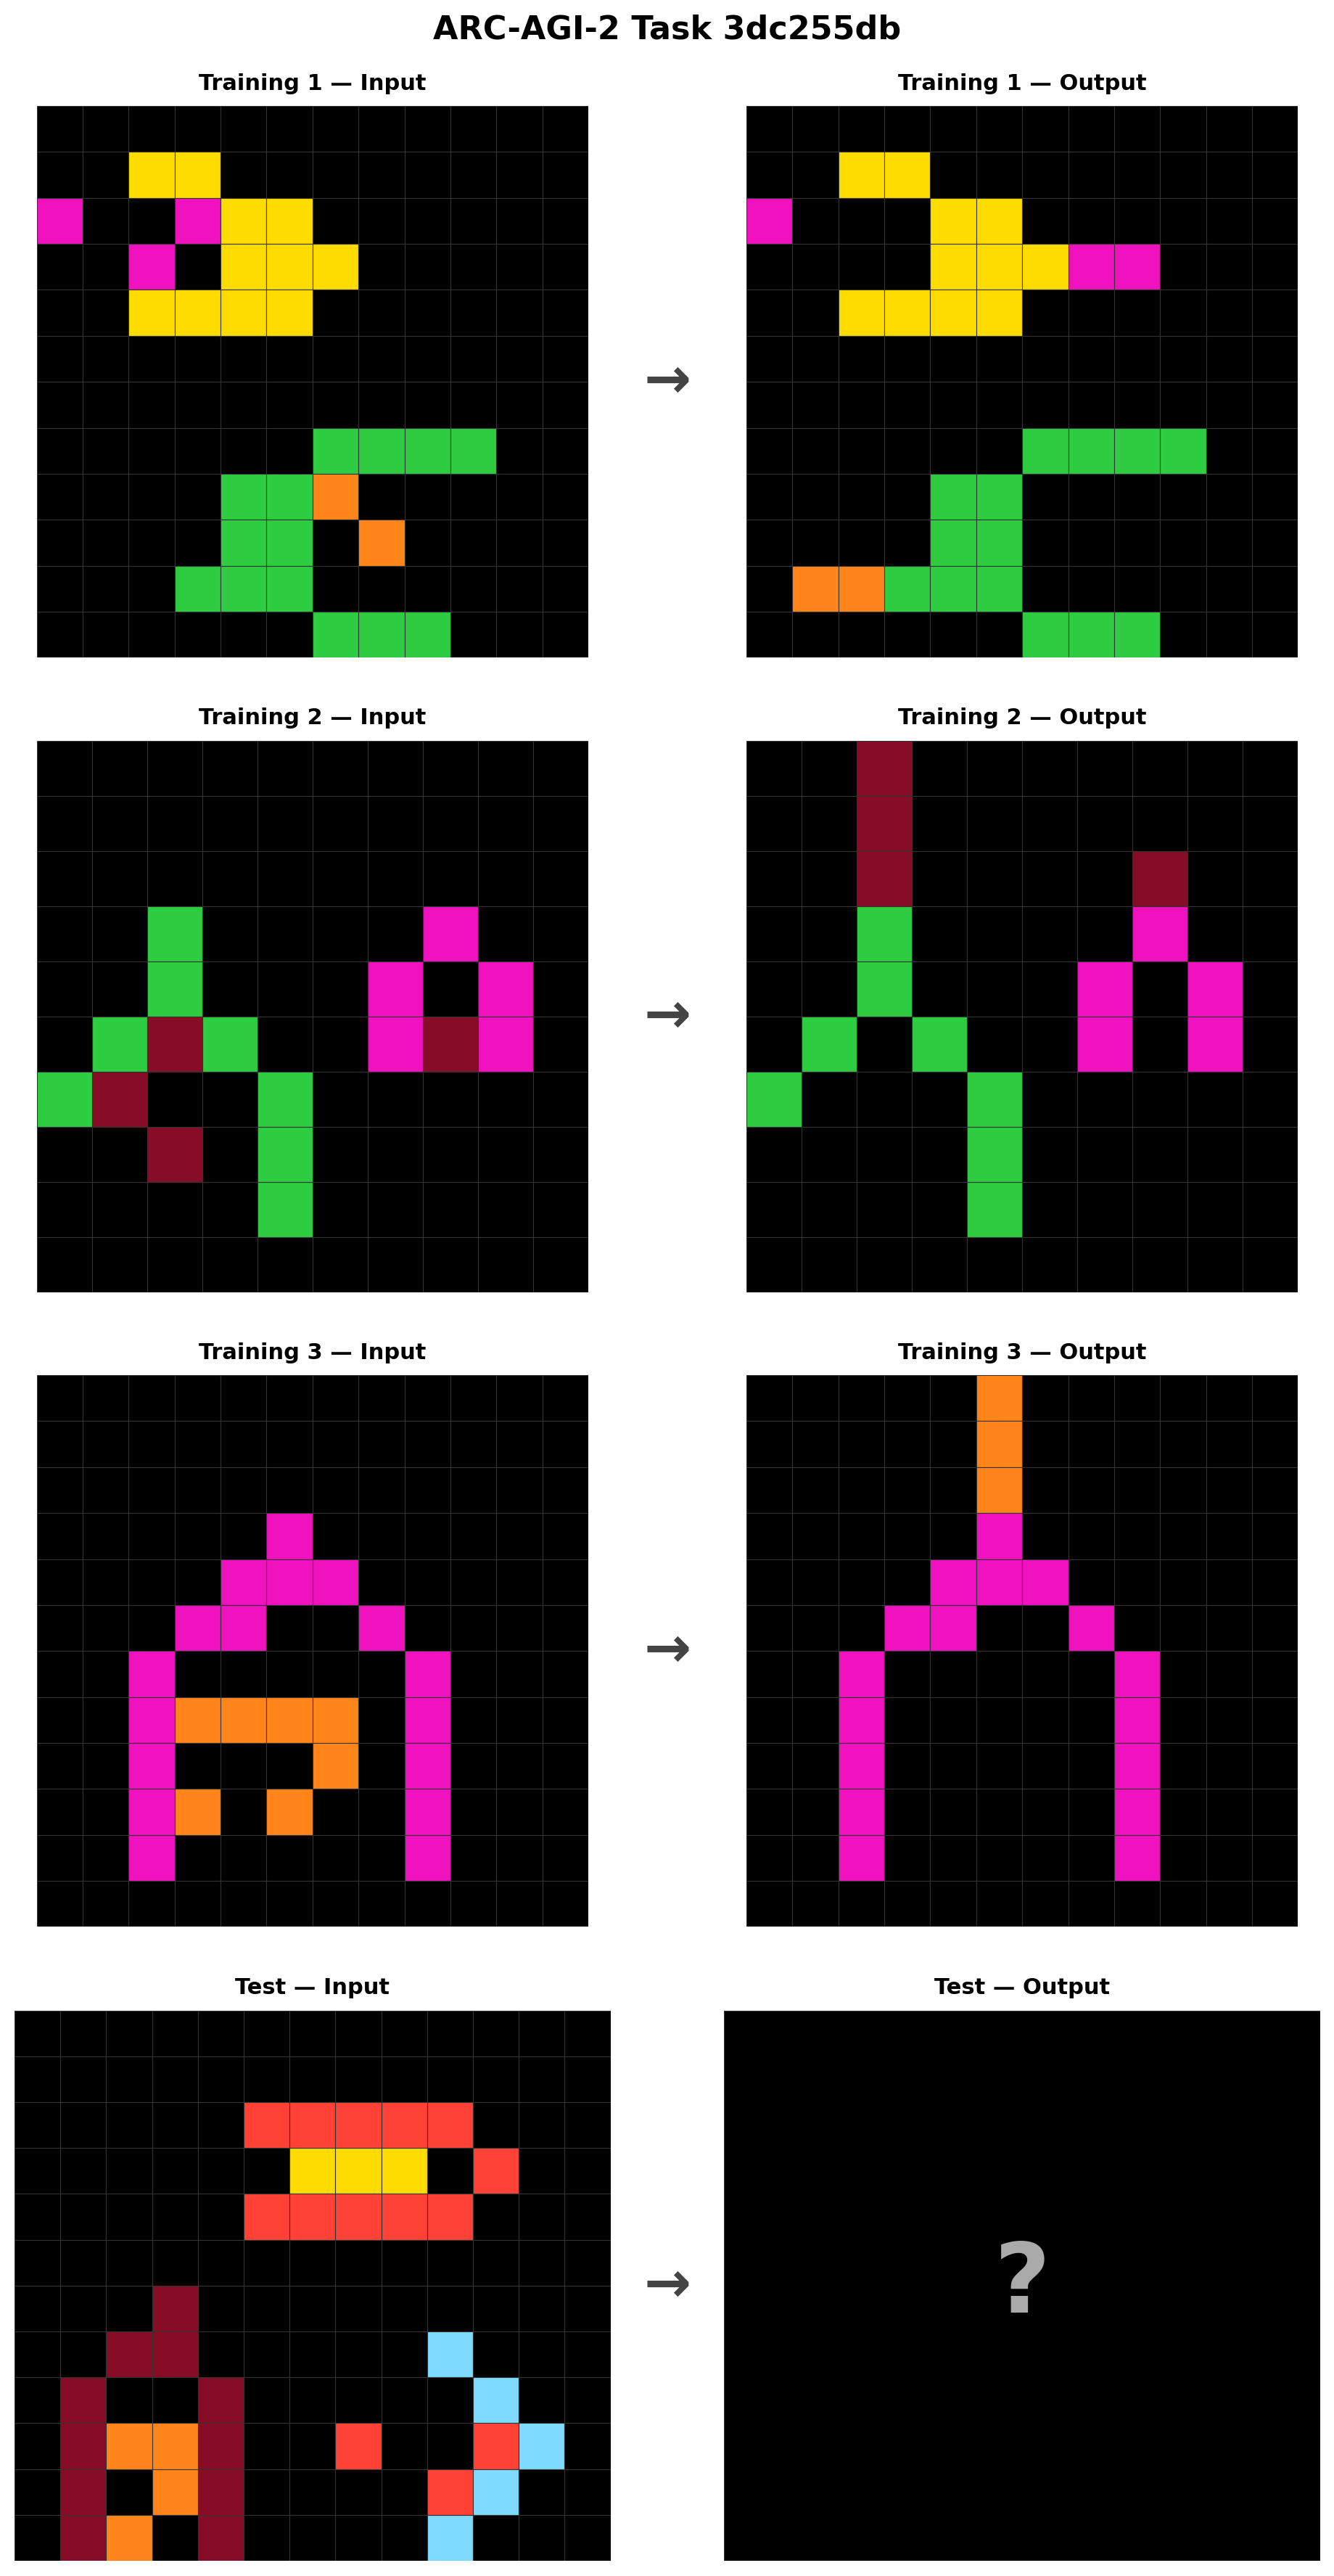
\includegraphics{figures/task_example.png}
\caption{ARC-AGI-2 task \texttt{3dc255db}. Three training pairs (rows
1--3) demonstrate the rule; the test input (row 4) must be solved from
these examples alone.}
\end{figure}

\hypertarget{image-rendering-example}{%
\subsection{Image Rendering Example}\label{image-rendering-example}}

The figure below shows an example of the intentionally imprecise image
rendering used for image-based prompting. Each training pair is shown as
an input/output image pair, with the test input at the bottom. The
slight distortion encourages models to reason about shapes and spatial
relationships at a higher level of abstraction rather than falling back
to cell-by-cell numerical processing.

\begin{figure}
\centering
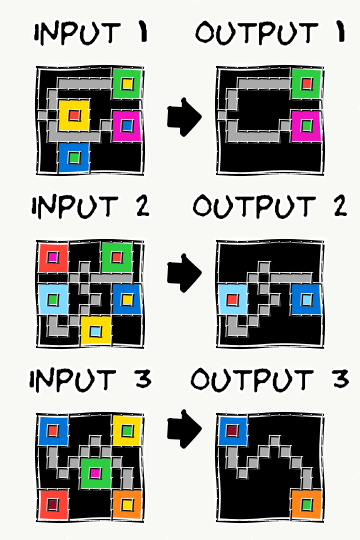
\includegraphics{figures/d35bdbdc_1_step_5_common.png}
\caption{Example image rendering used for image-based prompting (task
d35bdbdc:1).}
\end{figure}

\hypertarget{candidate-configuration-details}{%
\subsection{Candidate Configuration
Details}\label{candidate-configuration-details}}

Table 6 shows the full candidate configuration. The text family
contributes 8 candidates (including 4 deep-think runs), image
contributes 10, and code contributes 11. Within each family, multiple
runs of the same generator use the same prompt and API parameters;
diversity arises from model sampling stochasticity.

\begin{longtable}[]{@{}lll@{}}
\caption{Candidate configuration: 29 generators grouped by
family.}\tabularnewline
\toprule\noalign{}
Family & Generator & Candidates \\
\midrule\noalign{}
\endfirsthead
\toprule\noalign{}
Family & Generator & Candidates \\
\midrule\noalign{}
\endhead
\bottomrule\noalign{}
\endlastfoot
Text & Claude Opus 4.5 (text) & 1 \\
Text & Gemini 3 Preview (text) & 1 \\
Text & GPT-5.2 (text) & 2 \\
Text & GPT-5.2 (deep think) & 4 \\
Image & Gemini 3 Preview (image) & 4 \\
Image & GPT-5.2 (image) & 6 \\
Code & Gemini 3 Preview (code, tools) & 2 \\
Code & GPT-5.2 (code, tools) & 9 \\
& \textbf{Total} & \textbf{29} \\
\end{longtable}

\hypertarget{text-prompting-details}{%
\subsection{Text Prompting Details}\label{text-prompting-details}}

The base prompt is intentionally minimal:

\begin{Shaded}
\begin{Highlighting}[]
\NormalTok{You are solving an ARC (Abstraction and Reasoning Corpus)}
\NormalTok{task. Each grid cell is an integer 0{-}9 representing a color.}
\NormalTok{Use the solved examples to infer the transformation and}
\NormalTok{apply it to the test input.}
\NormalTok{...}
\NormalTok{\{training and test examples\}}
\NormalTok{...}
\NormalTok{Respond with an explanation of your thinking that is detailed}
\NormalTok{enough that someone can reconstruct your solution. Afterwards,}
\NormalTok{you MUST also respond with the completed output grid.}
\end{Highlighting}
\end{Shaded}

The prompt deliberately does \textbf{not} prescribe a fixed reasoning
template, a step-by-step plan, or a fixed output grid format. This
reduces ``prompt compliance'' overhead and empirically increases
hypothesis diversity. The trade-off is that outputs are noisier and
require tolerant parsing and validation to recover candidate grids (see
Section 6 for supporting negative results on strict output constraints).

Grids are encoded in \textbf{CSV format}, which was selected after
benchmarking 9 representation formats (standard space-separated,
semicolon-delimited, XML-tagged, CSV, Python lists, sparse coordinate
notation, ASCII symbols, binary masks, and compact pipe-delimited).
Suboptimal format choices cost on the order of 10\% lost performance
relative to CSV, with compact formats that are difficult for LLMs to
produce (e.g., sparse coordinate notation, binary masks) performing
substantially worse.

\hypertarget{code-generation-trace-example}{%
\subsection{Code Generation Trace
Example}\label{code-generation-trace-example}}

The tool-integrated code generation regime often produces rich
intermediate artifacts (program drafts, test harnesses, and execution
traces) that are later consumed by the holistic judge. A shortened
excerpt of the tool-integrated trace illustrates the iterative
development pattern:

\begin{Shaded}
\begin{Highlighting}[]
\NormalTok{"detailed\_logs": [}
\NormalTok{  \{}
\NormalTok{    "type": "code",}
\NormalTok{    "code": "import numpy as np, collections,}
\NormalTok{             itertools, math, sys, statistics\textbackslash{}n",}
\NormalTok{    "language": "python"}
\NormalTok{  \},}
\NormalTok{  ...}
\NormalTok{  \{}
\NormalTok{    "type": "code",}
\NormalTok{    "code": "\# Display expected outer right region}
\NormalTok{             \# values for rows0{-}19 cols9{-}19}
\NormalTok{             outer\_expected = ex1\_out[:,9:20]}
\NormalTok{             outer\_pred = pred1[:,9:20]}
\NormalTok{             outer\_in = ex1\_in[:,9:20]}
\NormalTok{             outer\_expected.shape\textbackslash{}n",}
\NormalTok{    "language": "python"}
\NormalTok{  \},}
\NormalTok{  ...}
\NormalTok{  \{}
\NormalTok{    "type": "code",}
\NormalTok{    "code": "\# Let\textquotesingle{}s craft final version and re{-}test.}
\NormalTok{             import numpy as np}
\NormalTok{             from collections import Counter, deque}

\NormalTok{             def solver(input\_grid):}
\NormalTok{                 g = np ...\textbackslash{}n",}
\NormalTok{    "language": "python"}
\NormalTok{  \},}
\NormalTok{  \{}
\NormalTok{    "type": "text",}
\NormalTok{    "content": "\#\#\# FINAL SOLUTION \#\#\#}
\NormalTok{               import numpy as np}
\NormalTok{               from collections import Counter, deque}

\NormalTok{               def solver(input\_grid):}
\NormalTok{                   g = np.array(input\_grid, ...)}
\NormalTok{                   h, w = g ..."}
\NormalTok{  \}}
\NormalTok{]}
\end{Highlighting}
\end{Shaded}

\hypertarget{judge-prompt-structure}{%
\subsection{Judge Prompt Structure}\label{judge-prompt-structure}}

The holistic judge prompt is assembled programmatically and follows this
structure (condensed; the full implementation is in the released source
code {[}anonymized for review{]}):

\begin{Shaded}
\begin{Highlighting}[]
\NormalTok{Below is a problem that was attempted to be solved \{N\} times:}

\NormalTok{\{training pairs + test input\}}

\NormalTok{Solutions were generated \{N\} times, using different types of solvers.}

\NormalTok{\textless{}SOLUTION 1 START\textgreater{}}
\NormalTok{\textless{}CONTENT\textgreater{}}
\NormalTok{\{full reasoning trace or extracted solver function\}}
\NormalTok{\textless{}/CONTENT\textgreater{}}
\NormalTok{\textless{}PREDICTED\_GRID\textgreater{}}
\NormalTok{\{candidate output as CSV\}}
\NormalTok{\textless{}/PREDICTED\_GRID\textgreater{}}
\NormalTok{\textless{}SOLUTION 1 STOP\textgreater{}}

\NormalTok{... (repeated for all N solutions) ...}

\NormalTok{Your task is to understand these solutions, and assess how well they\textquotesingle{}ve}
\NormalTok{understood the problem, and how likely their solutions are to provide the}
\NormalTok{correct solution to the test input.}

\NormalTok{Often, new mechanics are introduced in the test example for which the}
\NormalTok{solutions do not generalize well. Please output two solutions that you}
\NormalTok{think represent the right mechanic for solving the problem.}

\NormalTok{Output your two solutions as grids (in code blocks). Explain how you}
\NormalTok{came to these two solutions being the two most likely. Study all the}
\NormalTok{provided solutions and their reasoning to come up with a meta{-}conclusion}
\NormalTok{about how to solve the problem.}
\end{Highlighting}
\end{Shaded}

Each candidate's \texttt{CONTENT} block contains the full reasoning
trace --- for text/image candidates this is the model's chain-of-thought
response, and for code candidates it is the complete iterative tool-use
trace including intermediate program drafts, execution outputs, and
debugging steps. Candidates that produce identical output grids are
listed as separate solutions (with separate traces), preserving the
judge's ability to assess reasoning quality even when outputs agree.

\hypertarget{failure-analysis-generation-failures-21-instances}{%
\subsection{Failure Analysis: Generation Failures (21
instances)}\label{failure-analysis-generation-failures-21-instances}}

The following instances have zero correct candidates across all
modalities (with full 29-candidate coverage):

\begin{longtable}[]{@{}lll@{}}
\toprule\noalign{}
Task & Test & Link \\
\midrule\noalign{}
\endhead
\bottomrule\noalign{}
\endlastfoot
\texttt{21897d95} & 1 & https://arcprize.org/play?task=21897d95 \\
\texttt{2b83f449} & 1 & https://arcprize.org/play?task=2b83f449 \\
\texttt{3a25b0d8} & 1 & https://arcprize.org/play?task=3a25b0d8 \\
\texttt{3dc255db} & 1 & https://arcprize.org/play?task=3dc255db \\
\texttt{4c416de3} & 1 & https://arcprize.org/play?task=4c416de3 \\
\texttt{4e34c42c} & 2 & https://arcprize.org/play?task=4e34c42c \\
\texttt{5545f144} & 1 & https://arcprize.org/play?task=5545f144 \\
\texttt{6ffbe589} & 1 & https://arcprize.org/play?task=6ffbe589 \\
\texttt{88e364bc} & 1 & https://arcprize.org/play?task=88e364bc \\
\texttt{8b7bacbf} & 1 & https://arcprize.org/play?task=8b7bacbf \\
\texttt{8b7bacbf} & 2 & https://arcprize.org/play?task=8b7bacbf \\
\texttt{9bbf930d} & 1 & https://arcprize.org/play?task=9bbf930d \\
\texttt{a25697e4} & 1 & https://arcprize.org/play?task=a25697e4 \\
\texttt{abc82100} & 1 & https://arcprize.org/play?task=abc82100 \\
\texttt{b9e38dc0} & 1 & https://arcprize.org/play?task=b9e38dc0 \\
\texttt{d35bdbdc} & 2 & https://arcprize.org/play?task=d35bdbdc \\
\texttt{da515329} & 1 & https://arcprize.org/play?task=da515329 \\
\texttt{de809cff} & 1 & https://arcprize.org/play?task=de809cff \\
\texttt{e12f9a14} & 1 & https://arcprize.org/play?task=e12f9a14 \\
\texttt{e12f9a14} & 2 & https://arcprize.org/play?task=e12f9a14 \\
\texttt{faa9f03d} & 1 & https://arcprize.org/play?task=faa9f03d \\
\end{longtable}

\hypertarget{failure-analysis-selection-failures-17-instances}{%
\subsection{Failure Analysis: Selection Failures (17
instances)}\label{failure-analysis-selection-failures-17-instances}}

The following instances have at least one correct candidate, but the
holistic judge fails to select it:

\begin{longtable}[]{@{}lll@{}}
\toprule\noalign{}
Task & Test & Link \\
\midrule\noalign{}
\endhead
\bottomrule\noalign{}
\endlastfoot
\texttt{16b78196} & 1 & https://arcprize.org/play?task=16b78196 \\
\texttt{35ab12c3} & 1 & https://arcprize.org/play?task=35ab12c3 \\
\texttt{36a08778} & 2 & https://arcprize.org/play?task=36a08778 \\
\texttt{4c7dc4dd} & 1 & https://arcprize.org/play?task=4c7dc4dd \\
\texttt{4e34c42c} & 1 & https://arcprize.org/play?task=4e34c42c \\
\texttt{6e4f6532} & 1 & https://arcprize.org/play?task=6e4f6532 \\
\texttt{7666fa5d} & 1 & https://arcprize.org/play?task=7666fa5d \\
\texttt{78332cb0} & 1 & https://arcprize.org/play?task=78332cb0 \\
\texttt{78332cb0} & 2 & https://arcprize.org/play?task=78332cb0 \\
\texttt{7b80bb43} & 1 & https://arcprize.org/play?task=7b80bb43 \\
\texttt{88bcf3b4} & 2 & https://arcprize.org/play?task=88bcf3b4 \\
\texttt{89565ca0} & 1 & https://arcprize.org/play?task=89565ca0 \\
\texttt{9aaea919} & 1 & https://arcprize.org/play?task=9aaea919 \\
\texttt{a32d8b75} & 1 & https://arcprize.org/play?task=a32d8b75 \\
\texttt{d35bdbdc} & 1 & https://arcprize.org/play?task=d35bdbdc \\
\texttt{e3721c99} & 2 & https://arcprize.org/play?task=e3721c99 \\
\texttt{eee78d87} & 1 & https://arcprize.org/play?task=eee78d87 \\
\end{longtable}

\hypertarget{judge-transcript-examples}{%
\subsection{Judge Transcript Examples}\label{judge-transcript-examples}}

\hypertarget{minority-recovery-dfadab011}{%
\subsubsection{\texorpdfstring{Minority recovery:
\texttt{dfadab01:1}}{Minority recovery: dfadab01:1}}\label{minority-recovery-dfadab011}}

This instance heavily suffers from ``group think'': 12 of the candidate
solvers converge on the same incorrect output, and another 8 converge on
a second incorrect output. Only one candidate solver produces the
correct output. The judges identify the originality in this lone
solution and select it:

\begin{Shaded}
\begin{Highlighting}[]
\NormalTok{Most candidate solvers correctly identify the}
\NormalTok{core stamp mechanic:}
\NormalTok{...}
\NormalTok{I prefer solutions that do *not* stamp at (9,8)}
\NormalTok{(e.g., solutions 10{-}15/17{-}20) over those that}
\NormalTok{stamp every 8.}

\NormalTok{The only remaining ambiguity is edge handling}
\NormalTok{(not clearly disambiguated by the training set):}
\NormalTok{{-} Some solvers assume a stamp must fit fully}
\NormalTok{  (ignore row 17 markers).}
\NormalTok{{-} Others assume stamps are clipped at the border}
\NormalTok{  (row 17 markers produce the top 3 rows of}
\NormalTok{  the tile).}

\NormalTok{So the two most plausible outputs}
\NormalTok{(same mechanic, differing only in border handling)}
\end{Highlighting}
\end{Shaded}

The judge correctly identifies that the core mechanic is not in dispute
and reasons that the real ambiguity lies in edge handling. Rather than
committing both guesses to the majority interpretation, the judge uses
the pass@2 format to hedge: it selects one output for each
interpretation of the border behavior.

\hypertarget{synthesis-example-21897d952}{%
\subsubsection{\texorpdfstring{Synthesis example:
\texttt{21897d95:2}}{Synthesis example: 21897d95:2}}\label{synthesis-example-21897d952}}

This is a particularly difficult task where \textbf{none} of the 29
candidates produced a correct output. The judge synthesized a correct
output by recombining partial insights from multiple flawed candidates:

\begin{Shaded}
\begin{Highlighting}[]
\NormalTok{{-}{-}{-} COUNCIL OF JUDGES SYNTHESIZED SOLUTION {-}{-}{-}}
\NormalTok{Across the training examples, the only solutions that}
\NormalTok{consistently match the *actual* structure are SOLUTION 1}
\NormalTok{and SOLUTION 2 (they are the same). They correctly}
\NormalTok{identify the key mechanic:}

\NormalTok{{-} The input is divided into large "rooms" (rectangular}
\NormalTok{  regions of a dominant background color).}
\NormalTok{{-} Inside rooms, color 1 forms a 4{-}cell T{-}shape arrow}
\NormalTok{  (a 3{-}long bar + 1{-}cell stem).}
\NormalTok{{-} The stem direction indicates which neighboring room}
\NormalTok{  is the target.}
\NormalTok{{-} The paint color is:}
\NormalTok{  {-} the center of the 3{-}long bar if it is not 1}
\NormalTok{    (a payload color), otherwise}
\NormalTok{  {-} the background color of the room containing}
\NormalTok{    the arrow.}
\NormalTok{...}
\NormalTok{the same room recoloring but then rotated 90 CCW.}
\NormalTok{This is much less likely given the square training}
\NormalTok{examples, but it matches the extra rotation behavior}
\NormalTok{seen in the non{-}square examples and is the most}
\NormalTok{plausible "geometry variant" if a solver applied}
\NormalTok{that step unconditionally}
\NormalTok{...}
\end{Highlighting}
\end{Shaded}

\hypertarget{selection-failure-examples}{%
\subsection{Selection Failure
Examples}\label{selection-failure-examples}}

\textbf{\texttt{36a08778}} (test 2): The training examples establish a
straightforward ``water flows downward'' mechanic. Test 2 introduces
walls that block flow --- a new structural element not present in
training. Most candidates (and the judge) converge on the simpler
mechanic:

\begin{Shaded}
\begin{Highlighting}[]
\NormalTok{Most of the 29 solvers converged to the *same* mechanic (and the same output)}
\NormalTok{...}
\NormalTok{I discarded outliers like **Solution 2** and **Solution 1**}
\end{Highlighting}
\end{Shaded}

\textbf{\texttt{88bcf3b4}} (test 2): Training examples show a single
``rope/snake'' component moving in one direction. Test 2 introduces
multiple strings moving in multiple directions. The judge identifies the
ambiguity but cannot resolve it:

\begin{Shaded}
\begin{Highlighting}[]
\NormalTok{From the 5 training examples, the consistent mechanic is **not** "gravity" or}
\NormalTok{"attraction" of whole blobs. Instead, one non{-}background component acts like a}
\NormalTok{**rope/snake**}
\NormalTok{...}
\NormalTok{The main ambiguity the examples do *not* disambiguate is what happens when the}
\NormalTok{"returning" segment reaches the pole\textquotesingle{}s column/row again}
\end{Highlighting}
\end{Shaded}

\hypertarget{candidate-generation-cost-by-modality}{%
\subsection{Candidate Generation Cost by
Modality}\label{candidate-generation-cost-by-modality}}

\begin{longtable}[]{@{}llll@{}}
\caption{Candidate generation cost by modality family.}\tabularnewline
\toprule\noalign{}
Modality family & Total (\$) & Avg \$/instance & \% of generation
cost \\
\midrule\noalign{}
\endfirsthead
\toprule\noalign{}
Modality family & Total (\$) & Avg \$/instance & \% of generation
cost \\
\midrule\noalign{}
\endhead
\bottomrule\noalign{}
\endlastfoot
Text (incl.~deep think) & 597.70 & 3.58 & 28.7\% \\
Image & 467.10 & 2.80 & 22.5\% \\
Code & 1016.56 & 6.09 & 48.9\% \\
\end{longtable}

\hypertarget{modality-ablations-oracle-level}{%
\subsection{Modality Ablations
(Oracle-Level)}\label{modality-ablations-oracle-level}}

Section 4 reports modality-level uniqueness on the
\textbf{complete-coverage subset} (n = 130), where all modalities are
executed. In this subset, the following \textbf{exclusive} oracle
solvability counts are observed (Table 3): Text only = 2, Image only =
6, Code only = 7. These exclusive counts imply that removing any single
modality would reduce candidate-oracle coverage by at least a few
percent.

However, oracle-level analysis has an important limitation: it measures
whether a correct candidate \emph{exists} in a modality's output, but
does not measure the end-to-end effect of removing that modality on the
final system output. Removing a modality could affect judge behavior in
ways not captured by oracle overlap --- for instance, reducing the
number of candidates changes cluster dynamics, which could make it
easier or harder for the holistic judge to identify the correct
solution.

The proper ablation --- running the full pipeline with one modality
family removed and re-running judging on the reduced candidate pool ---
has not been performed. The oracle-level uniqueness numbers should be
interpreted as a lower bound on each modality's contribution, not as a
precise end-to-end attribution.

\hypertarget{unperformed-ablations-1}{%
\subsection{Unperformed Ablations}\label{unperformed-ablations-1}}

The following ablations would strengthen the paper's claims but have not
been run due to cost constraints.

\textbf{Generation ablations:}

\begin{itemize}
\tightlist
\item
  \textbf{End-to-end modality removal:} run the full pipeline with one
  modality family removed and re-run judging on the reduced candidate
  pool. This requires at minimum three full runs (\textasciitilde\$7,200
  total).
\item
  \textbf{Independent candidates vs sequential refinement:} hold compute
  fixed and compare N independent candidates against N sequential
  refinement steps.
\item
  \textbf{Candidate budget scaling:} sweep the number of candidates per
  modality/model to estimate marginal returns per additional candidate.
\item
  \textbf{Per-model contribution:} isolate the contribution of each
  foundation model by running the pipeline with one model removed
  entirely.
\item
  \textbf{Temperature and sampling parameters:} sweep temperature,
  top-p, and other sampling parameters within each modality.
\item
  \textbf{Representation formats:} CSV vs alternative encodings,
  evaluated under the same candidate/judge budgets.
\end{itemize}

\textbf{Selection and judging ablations:}

\begin{itemize}
\tightlist
\item
  \textbf{Full majority-vote baseline comparison:} run majority vote as
  the sole selection mechanism in a full end-to-end run.
\item
  \textbf{Judge ensemble sizing:} compare 1-judge vs 3-judge accuracy.
\item
  \textbf{Alternative selection mechanisms:} compare against per-output
  log-probability scoring, pairwise tournaments, and best-of-N with a
  reward model.
\item
  \textbf{Judge model diversity:} rigorously compare homogeneous vs
  mixed-model judge ensembles.
\item
  \textbf{Trace content ablation:} compare judge accuracy with traces vs
  outputs-only.
\end{itemize}

\textbf{Early stopping ablations:}

\begin{itemize}
\tightlist
\item
  \textbf{Early stopping threshold tuning:} vary the agreement threshold
  and the number of candidates consulted before the stopping decision.
\end{itemize}

\hypertarget{negative-results-full-details}{%
\subsection{Negative Results: Full
Details}\label{negative-results-full-details}}

\hypertarget{hint-generation-followed-by-solver-discarded}{%
\subsubsection{Hint generation followed by solver
(discarded)}\label{hint-generation-followed-by-solver-discarded}}

This approach is structurally similar to iterative self-improvement
methods such as Self-Refine \citep{madaan2023selfrefine} and Reflexion
\citep{shinn2023reflexion}. The hint stage often \textbf{limits
creativity} and collapses candidate diversity into a narrower space,
which is counterproductive when trying to break new ground.

\hypertarget{object-identification-followed-by-transformation-identification-followed-by-solver-discarded}{%
\subsubsection{Object identification followed by transformation
identification followed by solver
(discarded)}\label{object-identification-followed-by-transformation-identification-followed-by-solver-discarded}}

Structured decomposition to ``force'' abstraction. Failure mode: brittle
handoff between stages. Both verbose and overly terse handovers caused
confusion and reduced diversity, often regressing toward the mean rather
than expanding the hypothesis space.

\hypertarget{opus-codegen-and-opus-image-reasoning-discarded-from-final-mix}{%
\subsubsection{Opus codegen and Opus image reasoning (discarded from
final
mix)}\label{opus-codegen-and-opus-image-reasoning-discarded-from-final-mix}}

Opus contributes only a single text-reasoning candidate in the final
system. Opus codegen and image reasoning were tested but contributed
less uniquely relative to the GPT/Gemini configurations.

\hypertarget{grid-representations-and-output-constraints-discarded-variants}{%
\subsubsection{Grid representations and output constraints (discarded
variants)}\label{grid-representations-and-output-constraints-discarded-variants}}

CSV-style encoding outperformed many alternatives, especially as grids
grow. Forcing strict outputs (e.g., requiring JSON via API-level
response formats) underperformed. Removing constraints increases output
noise; robust parsing (regex + validation) becomes necessary, but was
worth it for accuracy.

\hypertarget{synthetic-data-augmentation-for-code-candidates-discarded}{%
\subsubsection{Synthetic data augmentation for code candidates
(discarded)}\label{synthetic-data-augmentation-for-code-candidates-discarded}}

Surface-level augmentations (color permutation) add little signal.
Geometric transforms (rotation, mirroring) break semantics for
orientation-dependent tasks. Meaningful augmentation requires solving
the task first --- making it infeasible in a private-dataset evaluation
setting.

\hypertarget{extensive-prompt-engineering-discarded}{%
\subsubsection{Extensive prompt engineering
(discarded)}\label{extensive-prompt-engineering-discarded}}

The more prescriptive the prompt, the worse the system performed on the
hardest tasks. The mechanism appears to be a \textbf{compliance tax on
reasoning}: when the model is given detailed instructions about
\emph{how} to think, it allocates reasoning budget to following those
instructions rather than to actually solving the problem. Tested
strategies included prescribed reasoning templates, structured output
requirements, detailed chain-of-thought scaffolding, domain-specific
heuristics in the prompt, and iterative prompt refinement. In every
case, the final minimal prompt outperformed.

This also interacts with diversity: a prescriptive prompt narrows the
hypothesis space across candidates. When all N candidates follow the
same reasoning template, they tend to converge on the same (possibly
wrong) answer.

\bibliographystyle{tmlr}
\bibliography{refs}

\end{document}
